\section{Introducci\'on}

La configuraci\'on ''Darlington'', tambi\'en conocida como ''par Darlington'', consiste en dos transistores conectados como se observa en la figura \ref{darlington_ideal}, en colector común, con el fin de obtener una mayor ganancia de corriente respecto a la obtenida al emplear un \'unico transistor en la misma configuración. Se analiza el comportamiento del circuito para comprender la utilidad del par Darlington, muy utilizado como buffer, o seguidor de tensión. Se comienza por un an\'alisis te\'orico del circuito para luego implementarlo utilizando utilizando los transistores BC337-40.

\begin{figure}[H]
	\centering
		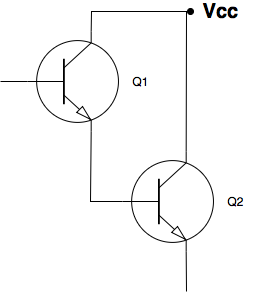
\includegraphics[scale=0.4]{./Imagenes/darlington_ideal.png} 
	\caption{Configuraci\'on Darlington.}
	\label{darlington_ideal}
\end{figure}
